\chapter{Zakłócenie w regulatorze DMC}
\label{zad5}
Poniżej (rys. \ref{fig:zak_bezr}) został zaprezentowany przebieg, w którym po osiągnięciu wartości zadanej, w chwili $k=100$ następuje skokowy wzrost zakłócenie z $0$ na $1$.

\begin{figure}[h!]
	\centering
	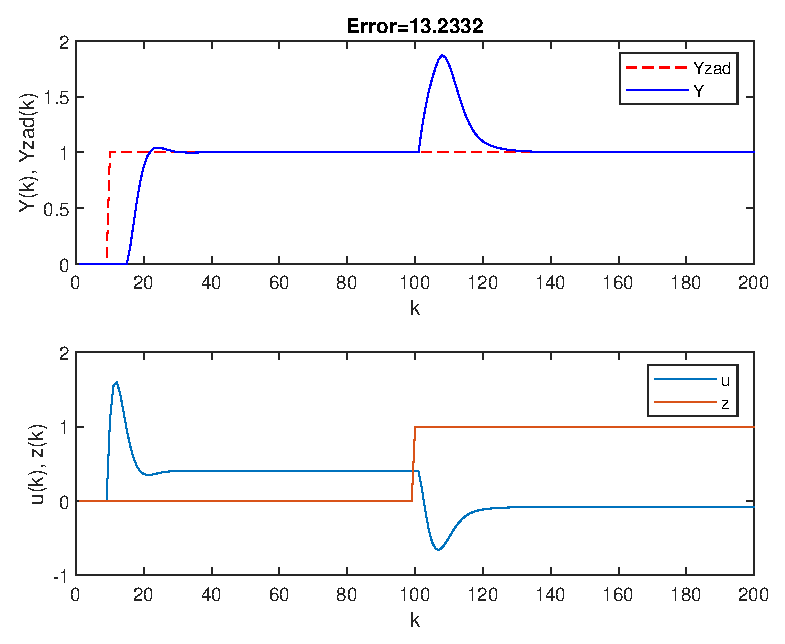
\includegraphics[scale=1]{Rys/zak_bezr.eps}
	\caption{Przebieg bez uwzględniania zakłócenia w regulacji}
	\label{fig:zak_bezr}
\end{figure}

\section{Dobór parametru $D_z$}
Prametr $D_z$ został dobrany, podobniej jak inne, za pomącą funkcji \verb|ga|. Poszykiwanie zostało przedstawione na wykresie \ref{fig:stojenie_dz}.

\begin{figure}[h!]
	\centering
	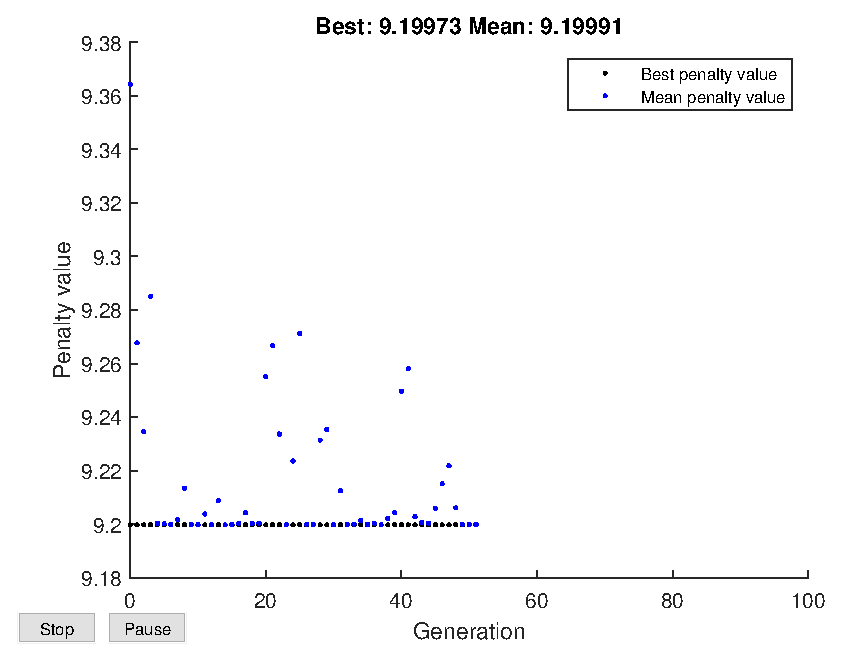
\includegraphics[scale=1]{Rys/strojenie_dz.eps}
	\caption{Poszukiwanie parametru $D_z$}
	\label{fig:stojenie_dz}
\end{figure}

Najlepszą jakość regulacji osiągnięto dla $D_z = 25$. Przebieg dla tej wartości można zobaczyć na wykresie \ref{fig:zak_zr}

\begin{figure}[h!]
	\centering
	\includegraphics[scale=1]{Rys/zak_zr.eps}
	\caption{Przebieg z uwzględnieniem zakłócenia w regulacji}
	\label{fig:zak_zr}
\end{figure}

\FloatBarrier

\section{Omówienie wyników}
Jak można zaobserwować na wykresach \ref{fig:zak_bezr} i \ref{fig:zak_zr} regulator biorący pod uwagę zakłócenie znacznie lepiej radzi sobie z zakłóceniem, szybciej wraca do wartości zadanej i zapobiega większym błędom.